% Author: Veena Iyer
%
% LLNCS macro package for Springer Computer Science proceedings;
% Version 2.21 of 2022/01/12
%
\documentclass[runningheads]{llncs}
%
\usepackage[T1]{fontenc}
% T1 fonts will be used to generate the final print and online PDFs,
%
\usepackage{graphicx}
% Used for displaying a sample figure. If possible, figure files should
% be included in EPS format.
%
% If you use the hyperref package, please uncomment the following two lines
% to display URLs in blue roman font according to Springer's eBook style:
\usepackage{hyperref} 
\usepackage{color}
\renewcommand\UrlFont{\color{blue}\rmfamily}
\urlstyle{rm}
%
% For display the content as it is mentioned
\usepackage{verbatim}

% Force figure placement with [H] option
\usepackage{float} 
%===============================================================================================%

\begin{document}
%
\title{Project Report}

\author{Veena Iyer}

\institute{University Freiburg, Freiburg, Germany}
%
\maketitle              

\section{Introduction}
The world of creating documents, papers, books, as well as plotting from simple to complex graphical plots have been enhanced and simplied by the introduction of {\LaTeX} and Gnuplot. These softwares enable people to focus on the real topic rather what is involved around them. 

I pesonally got inspired by these topics when they were dealt in the lecture as I found these topics very practical which can be used in the day-to-day technical applications.

In this report, we are going to discuss about various options explored with these softwares in detail and practically apply them for recreating a book and for generating readable graphs where there are several data involved.

%===============================================================================================%

\section{\LaTeX}
{\LaTeX} is a software system which is used for typesetting the documents. The document type can be a technical paper, book, article,resume, and the list is endless. The structure which {\LaTeX} uses for describing the content and the layout of how the document should look like is in the \textbf{markup} format. This is built on \TeX, which is a low-level typesetting language - initially designed for typesetting mathematical formulas and cross-referencing. 

There a various other tools available for document creation of which I had been using MS Word until I attended the lecture on \LaTeX. The differences I found between {\LaTeX} and conventional MS Word are written in Table 1.

\begin{table}
\caption{Main differences between \LaTeX and MS Word.} 
\begin{tabular}{p{0.49\linewidth}|p{0.49\linewidth}}
\multicolumn{1}{c|}{\LaTeX} & \multicolumn{1}{c}{MS Word} \\
\hline
Uses plain text along with markup tags for creating a document. & It is a grapical word processor based on WYSIWYG.\\
Compiled using  {\LaTeX} compiler for producing PDF. & No additional compiler needed. \\
Enables focus on the actual content (Scientific report writing, book creation, article generation). & Preferred for general purpose apllications, where it is possible to spend time in typesetting and formatting. \\
\end{tabular}
\end{table}

The differences listed in Table 1 acted as a strong base personally for me to shift from MS Word to {\LaTeX} for creating documents. Hence, as a first attempt in learning {\LaTeX}, several markups were looked into and were used for recreating a book.

%===============================================================================================%

\subsection{Method}
One of the first few book that I read as a child and which till date never fails to inspires me is the book APJ Abdul Kalam - Wings Of Fire, which is an autobiography written by Arun Tiwari as narrated by Dr. Kalam himself. I found this to be the most stuitable book to recreate in {\LaTeX} style and to demonstrate the {\LaTeX} commands that I learned. Only the original cover of the book was used for reference in the title page and rest of the contents were generated using the blindtext package and dummy images were used so as to preseve the originality of the book.

%===============================================================================================%

\subsection{Implemetation}
\subsubsection{Preamble : }
The document that is being recreated is a book. Hence, the \textbf{documentclass} was selected as \textbf{book}.
 
An insight of different packages that are used in recreation of the book are listed in Table 2.

\begin{table}
\centering
\caption{Packages used.} 
\begin{tabular}{{l|p{0.5\linewidth}}}
\multicolumn{1}{r|}{Package Name} & \multicolumn{1}{c}{Description}\\
\hline
babel & This document is created in English. Hence, conventional support related to formatting and structing are providing in English. \\
blindtext & Provides content for this book. \\
inputenc & For enabling proper interpretation and processing of text input using UTF-8 encoding. \\
titling & Used for customising the title page (title, author and maketitle).\\
titlesec & Used for customising the section, subsection commands. \\
graphicx & Enables to include images and customize them. \\
verbatim & Enables to display the content in the same format/structure as given. \\
xcolor & Provides different color options used in the document. \\
tikz & Provided support in the definition of custom styles used for the back cover page. \\
shadowtext & Enables the use of shadow effect used in the customised title page. \\
mathpazo & Provides different font options. \\
wrapfig & Enables placement of the figures in any desired part of a page. \\
\hline
\end{tabular}
\end{table}

With these packages used as the base, different commands are used for recreation of the book, where few self-motivated customization attempts have also been made. 

%===============================================================================================%

\subsubsection{Markup Commands : } 
The initial commands after the preamble section are general commands for checking if the {\LaTeX} syntax are in the latest style and to remove any extra pages, if any. 

'\texttt{\textbackslash definecolor{sandel}{HTML}{E6D6A8}}' \\
A color named as sandel has been created using HTML color code, which will later be used in the back title page.   

'\texttt{\textbackslash begin{document}}' and '\texttt{\textbackslash end{document}}' \\
These commands mark the beginning and end of the actual body of the book.

'\texttt{\textbackslash frontmatter}', '\texttt{\textbackslash mainmatter}' and '\texttt{\textbackslash backmatter}' \\
They are used to delineate the different sections of the book, and the appropriate content is placed within each section according to its purpose.

%===============================================================================================%

\subsubsection{Title Page : } 
The recreated book contains two title pages, of which the first title page contains the original cover of the book and the second one is the customised title page, where a different image with different sizing has been designed as seen in Fig.1. 

    \begin{figure}
    	\centering
    	\includegraphics[width=0.6\textwidth]{TitlePage.jpg}
    	\caption{Redesigned title page.}
    \end{figure}

The title of the book as in the Fig.1 is displayed by providing effects with a ´\texttt{\textbackslash shadowtext}´ which is created by controlling the x and y coordinates of the shadow with respect to the actual text. Also, different alignments, color options and spacing options for the texts are implemeted. 

%===============================================================================================%

\subsubsection{Headings Formatting : }
Following the design of title page, the formatting for each of the headings, like the parts and the chapters is done. Here, name of the parts are displayed on the center of the page in 'Huge' font in 'teal' color. {1em} is used for adding equal horizontal spaces before the name of the parts are displayed.

The names of the chapters are displayed in graycolor normal Huge font at the center. There is a vertical space of -2cm which is added before the chapter name. '\texttt{\textbraceleft\textbackslash huge\textbraceright[\textbackslash vspace\{1cm\}\textbackslash titlerule]}' - this sets a line below the name of every chapter before the start of the actual content. Spacing between the lines and the font size of the words are set using the '\texttt{\textbackslash linespread}' and '\texttt{\textbackslash fontsize}' commands, respectively.

%===============================================================================================%

\subsubsection{Content : }
In the original book, there is a poem written by Dr. Mr. Kalam which is recreated here using '\texttt{\textbackslash blindtext}'. Also, a dummy image (which is not in the book) is used for showing how the image can be displayed by cropping and in different angle. This is shown in the Fig.2.

\begin{figure}[H]
    \centering
    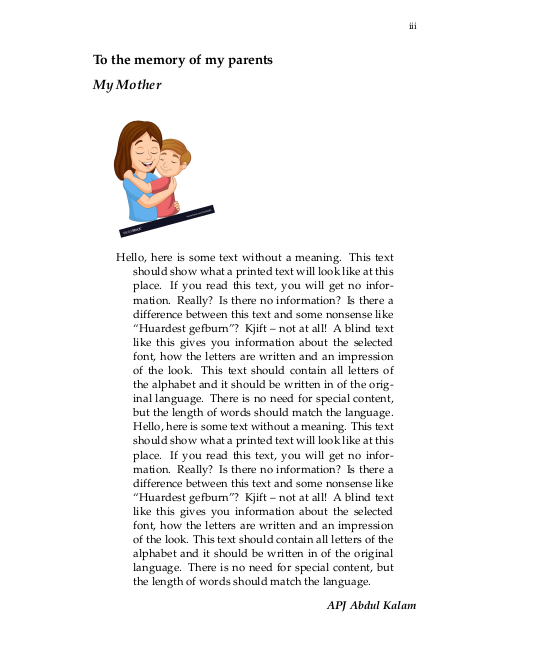
\includegraphics[width=0.5\textwidth]{Poem.jpg}
    \caption{Whole content is fitted in a single page.}
\end{figure}

As, seen in the Fig.2, these contents would have exceeded a single page, which is prevented by fitted in all the image, poem and the writer's name in single page by using the 'minipage' command. 

\begin{verbatim}
% minipage - used for having the whole content  
(image+poem+author name) in the same page
\begin{minipage}{\textwidth}
	\includegraphics[width=0.3\textwidth, clip, angle = 15]
	{mother-son.jpg}
\end{verbatim}

This page is followed by the table of content, which is recreated exactly like in the original book.

The chapters are begun after the table of contents page. There are few images in the original book, instead of which two other images are used to demonstarate the text wrapping feature and options available for placement of images in \LaTeX. 

Usage of different color for the content is demonstrated in the Epilogue page, where the content is displayed in violet color.

%===============================================================================================%

\subsubsection{Back Cover Page : }
In the actual book, the back page contains review from other people and the color of the page is sandel which is similar to the Fig.3. 

\begin{figure}[H]
    \centering
    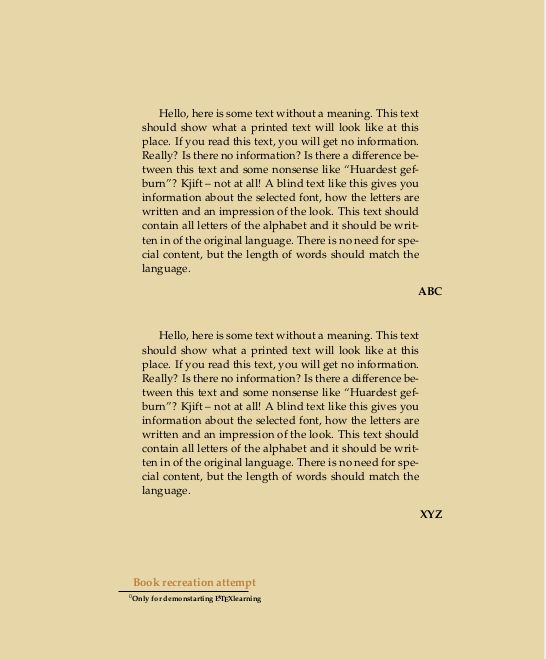
\includegraphics[width=0.6\textwidth]{BackPage.jpg}
    \caption{Recreated back cover page.}
\end{figure}

Here, as seen in Fig.3, in this recreation, the back page is given sandel color which is custom defined by HTML color code after the preamble section. Alignment of the the contents, footer notes have also been added which are similar to the original cover page.

%===============================================================================================%

\section{gnuplot}
The software I found very interesting for plotting is gnuplot, where any plot with any data can be generated. This is practically a very useful tool for every student as well as in technical fields as it can be used for a wide range of plotting applications. 

gnuplot is a command-line, a GUI program where it provides a wide range of options for different types of plots like 2D, 3D, histograms, plot of function, complex plots and the list is endless. In general the program is capable of accepting multiple data and it can also accept data from other live programs. In the upcoming sections, different plots that are generated by exploring options available in gnuplot. These options will be discussed in detail.  

%===============================================================================================%

\subsection{Method}
The topic gnuplot was deep discovered by creating 4 different plots, of which the first plot was a ternary plot, where different compositions of soil were taken as the data points. The Gnupot has no predefined functions for creating a triangle, which is the base for a ternary plot. Hence, by exploring different options, a triangle was created and the plotting of the data was done. To enhance the plot, colors for different compositions of the soil was given to the plot by diving the segments of the big triangle into smaller polygons, which prouced a combination of theses colors at the region where the different compositions of the soil merge.

For further plots, We have all seen weather report in NEWS channels and obsevered how colourful they are. In an attempt to explore options available for this, the next 3 plot are based on the average temperature of different cities from January to December from the year 1991 till 2020 were plotted. The cities are chosen from South pole to North pole, so that the temperature difference and weather pattern can be easily distinguishable. The plots represents these data but in different forms and in different readable styles. 

In the following sections, more details on the syntax for creating the plots are explained.

%===============================================================================================%

\subsection{Ternary Plot Implementation}
The basic condition for plotting a ternary plot is that, the sum of each row available in the data should be equal to 1 or 100. Only if this condition is met, the plot can be created. The data containing different compositions of soil satisfies this condition. 10 sample points were taken and the data was directly accessed by the code. The data contains the percentage composition of sand, silt, clay and color for each sample to be plotted. With this basic informations, a triangle was created in which the data will be plotted.

The raw data is initally converted into Cartesian coordinate system using trignometric folumae, which calculates the X and Y coordinates for the plot. Following this, the scales for the axes are set. For X-axis, the range is easy set from 0 to 100. But, for Y-axis, the range is set from 0 to $\frac{\sqrt{3}}{2}$ * 100, where $\frac{\sqrt{3}}{2}$ is the sin 60 and cos 30, which is used in the Cartesian coordinate conversion. All the angles used in this plot are in degree and hence changed from default radian unit. The code below would now be better understandible.

\begin{center}
\# Converting the data to Cartesian coordinate system for ternary plotting \\
\textit{xCoordinate(sand,silt,clay) = (sand + silt*cos(60))/(sand+silt+clay)*100} \\
\textit{yCoordinate(sand,silt,clay) = silt*cos(30) /(sand+silt+clay)*100} \\

\# Setting scale for X-axis \\
\textit{set xrange[0:100]} \\
\# Aspect ratio for the triangle \\
\textit{triangleRatio=(sqrt(3)/2)} \\
\# Setting size ratio for the triangle \\
\textit{set size ratio triangleRatio} \\
\# Setting the angles used in the ternary plot in degree instead of radian \\
\textit{set angle degrees} \\
\# Setting y-axis scale \\
\textit{set yrange[0:triangleRatio * 100]} \\ 
\end{center}

To make the plot readable, default commands for a 2D plot is unset and the plot is placed in such a point that it fits properly in the screen. The title for the plot is displayed with an offset in a visible font size without getting hindered by the plot. 

The ternary plot is divided into 6 ploygons based on their coordinates for applying different colors based on the actual color of the compositions. These colors a selected using HTML color code. The first 3 coordinates are for the base colors and the next 3 are polygons which have coordinates overlapping with 2 of the first 3 triangles. Here, it is expected to produce a different color when two of the three colors merge. From this, the color when all the 3 regions overlap is automatically produced, therby providing different color for different types of soil.

The colors, labels, angles and location of the labels on the sides of the triangle are customised with different options and formats. For readability of the plot, white dotted lines are used for the grid pattern. Here, a variable i is used as index, which gets incremented as the coordinates are covered. An unique identified for refering the arrows and grid lines inside the triangle is created as i+100, i+101, i+102, i+103, i+104 and i+105.

On the right side of the screen, the legend is printed, where the color and name of each point is displayed. Since this is not a normal plot, it was important to mention the dimensions for setting the legend, otherwise there would be an ovelap. The final commands generates a ternary plot with the mentioned legend.

%===============================================================================================%

\subsection{Temperature Plot Implementation}
Different plotting options are explored with the average temperature data across different cities in the world. These plots are explained below.

\subsubsection{Normal 2D Plot : }
Here, a normal 2D plot was generated by providing the data directly in the code. In this plot, options to set the X-axis label in different orientations have been tried out and the name of the months have been assigned as String type using 'set format x "\%s"' (instead of default numbers). Also, by default, the legend is set within the plot margin. Here, the option for setting it outside has been experimented. Also, each city is represented by different color and different point type so that they are easily readable.

\subsubsection{Contour Plot - 2D : }
The contour plot in 2D was aimed to generated a plot similar to heat map, where the temperatures are plotted based on the rgb shades according to their range. For doing this, it was important that the data are given in matrix format which is necessary for plotting a contour plot. This was done by storing the data in a .dat file. This file was then used for reading the data points. In this plot, both X and Y axis labels are provided in String format where the name of the months and the cities have been displayed. In this plot, the main learning was to set the intensity of colors according to requirement based on the shades of 'rgb' available in the gnuplot program. With these options, a colorful contour plot similar to a heat map was generated.

\subsubsection{Contour Plot - 3D : }
In order to venture more into options available in gnuplot related to contour plots, a 3D contour plot with the same average temperature data was plotted. In this plot, majority of the code was kept similar to the 2D contour plot and extra 3D feature was added. 'set hidden3d' displays the 3D countour plot and 'set pm3d at b' is used for placing the 2D contour plot at the bottom of the 3D plot. There are various options for placing the 2D plot like at the top or overlapping the 3D plot. The options that are best in terms of readabilty is used in the code.  

For the ease of generating the plots, a bash script was written (execute.sh), were all the four plots are genrated one after the other. By entering './execute.sh', all the plots can be viewed.

%===============================================================================================%

\section{Result}
\subsection{\LaTeX}
The book Wings of Fire was recreated by using different markup commands that are available in the document class for the type book. The typesetting, formatting, image sizing and placements, creation of new colors along with the available commands were explored and learnt.

\subsection{Gnuplot}
In gnuplot, different commands that are available for generating a good and readable graphs were deeply researched and most suitable ones were used. With various options, a triangular plot known as a ternary plot was generated in such a way that the data are clearly visible in a distinguishable manner, which is shown in Fig.4.

\begin{figure}[H]
    \centering
    \includegraphics[width=0.6\textwidth]{TernaryPlot.jpg}
    \caption{Output ternary plot.}
\end{figure}

With temperature data, serveral critical options which makes even a simple graph better understandable were explored. Fig. 5 shows a normal 2D graph.  

\begin{figure}[H]
    \centering
    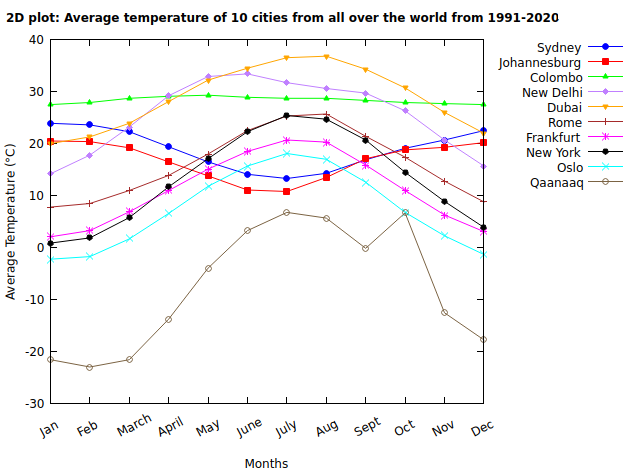
\includegraphics[width=0.6\textwidth]{Normal2D.jpg}
    \caption{Output of normal 2D plot.}
\end{figure}

The simplest graph to plot is 2D, in which different styles for each plot which has been designed, so that people with color-blindness can also understand the plot, was generated as in Fig.5. This was extended in a 2D contour plot with city and months as the axes labels as in Fig.6

\begin{figure}[H]
    \centering
    \includegraphics[width=0.6\textwidth]{Contour2D.jpg}
    \caption{Output of 2D contour plot.}
\end{figure}

As seen in Fig.6, a heat-map in the form of 2D contour with different color palatte for each temperature range was generated. After spending time on 2D plots, contour 3D plot was reseached, which is depicted in Fig.7.

\begin{figure}[H]
    \centering
    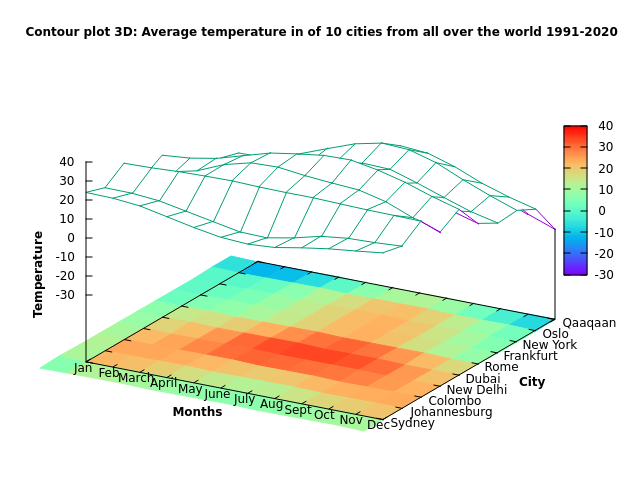
\includegraphics[width=0.6\textwidth]{Contour3D.jpg}
    \caption{Output of 3D contour plot.}
\end{figure}

Finally as in Fig.7, a 3D contour was plotted which was combined with the 2D contour plot, enabling people to see the pattern of weather across the cities.

Hence, while creating these plots, wide range of options available in gnuplot were delved deep into and most suitable options that makes a plot clean and readable were used in this project implementation.

%===============================================================================================%

\section{Conclusion}
Through this course and project implemetation, I personally have learned and gained confidence to in two very useful tools ({\LaTeX} and gnuplot) that I will from now on be using regularly. 

%===============================================================================================%

\begin{table}
\centering
\begin{tabular}{l p{0.5\linewidth}}
%\hline
Topics\\
\hline
Linux &  The project was done in Linux, but there is nothing special about it in this report\\
Text editor &  Nano was used for writing the codes for both {\LaTeX} and gnuplot. A small bash script was written using Nano for genrating all the plots together. \\
Git & Git was used as repository, but there is nothing to report it.\\
Docker & Not used. \\
Automation & Partially automated, only the execution the plots generated using Gnuplot were automated. \\
Gnuplot & One of the major topics of the project. Used for producing different types of graphs which is discussed in this report. \\
\LaTeX & Another topic of concentration in this project. Recreatation a book and and this report were both done in \LaTeX. \\
LLM & Not used.
%\hline
\end{tabular}
\caption{List of topics.}
\end{table}

%===============================================================================================%
%
% ---- Bibliography ----
%
% BibTeX users should specify bibliography style 'splncs04'.
% References will then be sorted and formatted in the correct style.
%
% \bibliographystyle{splncs04}
% \bibliography{mybibliography}
%
\begin{thebibliography}{8}
\bibitem{ref_url1}
LNCS Homepage, \url{http://www.springer.com/lncs}

\bibitem{ref_url2}
{\LaTeX} and gnuplot lecture slides (nextCloud), \url{https://nc.informatik.uni-freiburg.de}

\bibitem{ref_url3}
Gnuplot references, \url{http://www.gnuplot.info/demo/}

\bibitem{ref_url4}
Hexcode of different colors, \url{https://htmlcolorcodes.com/color-picker/}

\bibitem{ref_url5}
Average temperature of different cities, \url{https://www.climatestotravel.com/}

\bibitem{ref_url6}
Used for clarifying doubts from others questions, \url{https://tex.stackexchange.com/}

\end{thebibliography}
\end{document}
